\documentclass{article}
\usepackage{graphicx} % Required for inserting images
\usepackage{url}
\usepackage[T2A]{fontenc} % required for russian
\usepackage{hyphenat}
\hyphenation{}
\usepackage[english, russian]{babel}
\usepackage{gensymb}
\usepackage{amsmath}
\usepackage[a4paper, left=2cm, right=2cm, top=2cm, bottom=2cm]{geometry} % Adjust the margins here

\usepackage{wrapfig}
\usepackage{mathtext}
\usepackage{siunitx} % Required for alignment
\usepackage{subfigure}
\usepackage{multirow}
\usepackage{rotating}
\usepackage{afterpage}
\usepackage{caption}
\usepackage[arrowdel]{physics}
\usepackage{booktabs}

\begin{titlepage}
  \title{\textbf{Отчёт о выполнении лабораторной  работы 3.7.1} \\
                 Скин-эффект}
  \author{Балдин Виктор}
  \date{\today}
\end{titlepage}

\begin{document}
\maketitle
\newpage
\section{Аннотация:}
\noindent \textbf{Цель работы:}
\begin{enumerate}
  \item Исследовать явление проникновение переменного магнитного поля в медный полый цилиндр(скин эффект) % // TODO переформулировать
  \item Измерить проводимость меди 4 разными способами и сравних их
\end{enumerate}

\noindent \textbf{Методы измерений:}

\begin{enumerate}
    \item По наклону $1/\xi^2 $ от квадрата частоты
    \item По наклону тангенса сдвига фаз от частоты(при малых частотах)
    \item По наклону сдвига фаз от корня частоты(при больших частотах)
    \item По наклону функции мин-макс нормализации индуктивности от квадрата частоты
\end{enumerate}

\noindent\textbf{Приборы:} \\

\begin{enumerate}
    \item Генератор сигналов
    \item Соленоид
    \item Намотанный на полый цилиндрический каркас
    \item Медный экран в виде полого цилиндра
    \item Измерительная катушка
    \item Ам­перметр
    \item Вольтметр
    \item Двухканальный осциллограф
    \item RLC-метр
\end{enumerate}

% \begin{enumerate}
%     \item Генератор сигналов АКИП–3420ю
%     \item Соленоид
%     \item Намотанный на полый цилиндрический каркас
%     \item Медный экран в виде полого цилиндра
%     \item Измерительная катушка
%     \item Ам­перметр
%     \item Вольтметр
%     \item Двухканальный осциллограф GOS–620
%     \item RLC-метр
% \end{enumerate}

\newpage

% \section{Экспериментальная установка}


\section{Теоретические сведения}
% \subsection{Скин-эффект для полупрастранства}
% \vspace{1cm}

% \begin{wrapfigure}{l}{0.3\textwidth}
%   \begin{center}
%     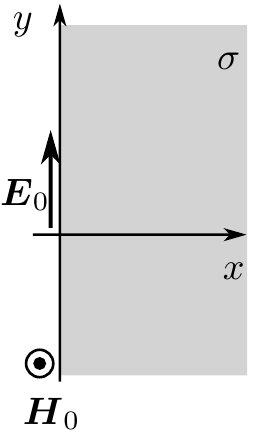
\includegraphics[width=0.28\textwidth]{poluprostranstvo}
%   \end{center}
%   \caption{Скин-эффект в полупространстве}\label{fig:poluprostranstvo}
% \end{wrapfigure}

% Рассмотрим квазистационарное поле внутри проводящей среды в простейшем плоском случае.
% Пусть вектор $\vb*{E}$ направлен всюду вдоль оси $y$ (рис.\ref{fig:poluprostranstvo})
% и зависит только от координаты $x$, т. е. ${E_x} = {E_z} \equiv 0$, $E_y=E_y(x,t)$.
% В квазистационарном приближении
% \begin{equation*}
%     \grad \times \vb*{H} = \sigma \vb*{E}
% \end{equation*}
% Берем ротор обоих частей
% \begin{equation*}
%     \grad \times (\grad \times \vb*{H}) = \grad(\grad \cdot \vb*{H}) - \grad^2\vb*{H} = \sigma \grad \times \vb*{E}
% \end{equation*}
% Испоьзуя ур-е Максвелла для ротора $\vb*{E}$ и для дивергенции $\vb*{H}$ получаем
% \begin{equation}
%     \grad^2 \vb*{H} = \sigma\mu\mu_0\frac{\partial\vb*{H}}{\partial t}
%                       + \grad(\grad \cdot \vb*{H}) = \sigma\mu\mu_0\frac{\partial\vb*{H}}{\partial t}
%     \label{eq:laplacian_H}
% \end{equation}
% Берем ротор еще раз
% \begin{equation*}
%     \grad \times (\grad^2\vb*{H}) = \grad^2 (\grad \times \vb*{H}) =
%     \sigma\mu\mu_0 \frac{\partial (\grad \times \vb*{H})}{\partial t}
% \end{equation*}
% Осталось подставить первое ур-е, и воспользоваться уравнением Максвелла
% \begin{equation}
%     \grad^2\vb*{E}=\sigma\mu\mu_0 \frac{\partial \vb*{E}}{\partial t}\label{eq:diffusion}
% \end{equation}

% Подставляем в (\ref{eq:diffusion}) наше электрическое поле $E_y=E_y(x,t)$
% \begin{equation}
%     \frac{\partial^2 E_y}{\partial x^2} = \sigma\mu\mu_0\frac{\partial E_y}{\partial t}
%     \label{eq:diffusion_chastni}
% \end{equation}
% Если $E_y(0,t)=E_0 e^{i\omega t}$ то решением (\ref{eq:diffusion_chastni}) будет функция вида
% \begin{equation}
%     E_y(x,t)=E_0 e^{-x/\delta} e^{i(\omega t - x/\delta)}
%     \label{eq:skin_effect_poluprostranstvo}
% \end{equation}
% где
% \begin{equation}
%     \delta = \sqrt{\frac{2}{\omega\sigma\mu\mu_0}}
%     \label{eq:delta}
% \end{equation}

% \newpage
\subsection{Скин-эффект в тонком полом цилиндре}
\vspace{1cm}
\begin{wrapfigure}[32]{l}{0.3\textwidth}
  \begin{center}
    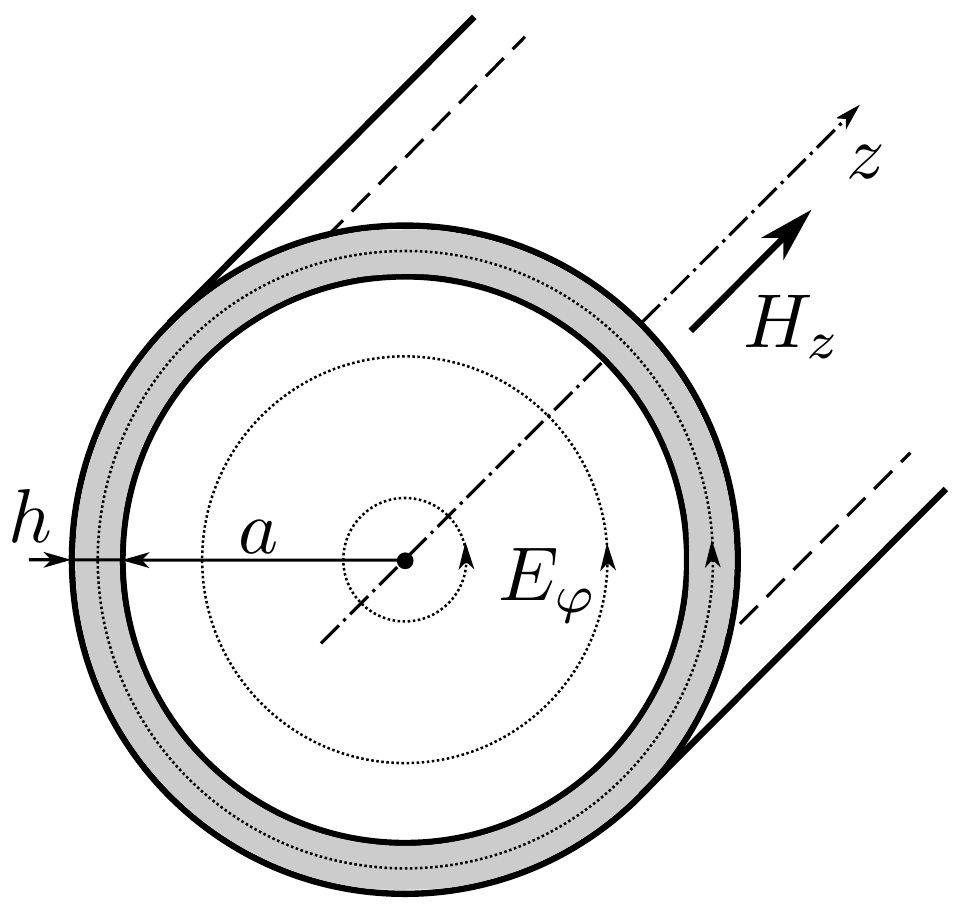
\includegraphics[width=0.28\textwidth]{cilindr}
  \end{center}
  \caption{Эл-магнитные поля в цилиндре}\label{fig:cilindr}

  \begin{center}
    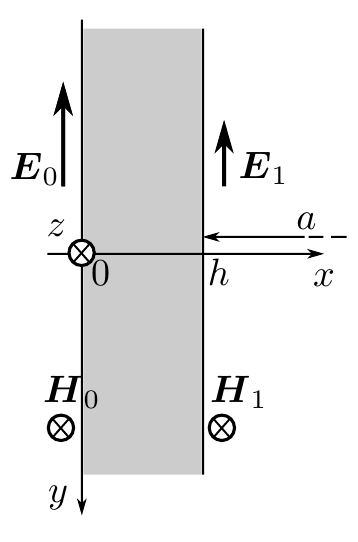
\includegraphics[width=0.28\textwidth]{stenka}
  \end{center}
  \caption{Стенка цилиндра}\label{fig:stenka}
\end{wrapfigure}

Рассмотрим длинный тонкостенном медном цилиндре. Из соображении симметрии и
непрерывности соответствующих компонент векторов $\vb*{E}$ и $\vb*{H}$ можем сказать что:
\begin{equation}
    H_z = H(r)e^{i\omega t} \text{, } E_\varphi = E(r)e^{i\omega t}
\end{equation}
и при этом функции $H(r)$ и $E(r)$ непрерывны.

Пусть цилиндр имеет радиус $a$ и толщину стенки $h \ll a$. Это позволяет для описания поля внутри стенки ограничится только одномерным приближением.

Внутри цилиндра токов нет, следовательно $H(r)=H_1=\text{const}$ внутри цилиндра.
По теореме об электромагнитной индукции в интегральной форме:
\begin{equation}
    E_{\varphi} \cdot 2 \pi r = - \mu_0 \pi r^2 \cdot \frac{dH_z}{dt} \quad \rightarrow \quad E(r) = -\frac{1}{2}\mu_0 r \cdot i \omega H_1
\end{equation}
откуда мы получаем граничное условие
\begin{equation}
    E_1=E(a)= -\frac{1}{2}i \omega a \mu_0 H_1
    \label{eq:granichnoe_uslovie_E}
\end{equation}

Поле внутри тонкой стенки цилиндра описывается уравнением скин-эффекта(л7.25) в плоской геометрии.

\begin{equation}
    \frac{d^2H}{dx^2} = i \omega \sigma \mu_0 H
\end{equation}

Граничные условия: $H_0 = H(0), \ H_1 = H(h)$

Решением будет:

% В приближении $h \ll a$ можем пренебречь кривизной стенки и смоделировать
% его бесконечной полосой. Тогда, надо решить уравнение (\ref{eq:laplacian_H})
% с граничными условиями. Решая уравнение получим связь полей $H_1$
% (поле внутри цилиндра которое мы будем измерять) и $H_2$, которое колебается с частотой
% $\omega$

\begin{equation}
    H_1 = \frac{H_0}{\ch(\alpha h) + \frac{1}{2} \alpha a \sh(\alpha h)} \quad \quad
    \alpha = \sqrt{i\omega \sigma \mu_0} = \frac{\sqrt{2}}{\delta}e^{i\pi/4}
    \label{eq:svyaz_poley}
\end{equation}

\vspace{4cm}
Рассмотрим предельные случае (2):

\textbf{Малые частоты} (от $~ 0.01\nu_h $ до $0.05\nu_h$):

\begin{equation}
    \frac{H_1}{H_0} = \frac{1}{1+\frac{1}{4}(ah\sigma \mu_0 \omega)^2} \quad \quad \xi = \xi_0  \frac{|H_1|}{|H_0|}
\end{equation}

\begin{equation}
    \frac{1}{\xi^2} = \frac{1}{\xi_0^2} \frac{1}{\left ( \frac{|H_1|}{|H_0|} \right )^2 } = \frac{1}{\xi_0^2} \left ( 1 + (\pi ah\sigma \mu_0 \nu)^2\right )
\end{equation}

или

\begin{equation}
    tg\psi = \frac{1}{2}ah\omega \sigma \mu_0
\end{equation}

\textbf{Большие частоты} (от $~ 0.05\nu_h $ до $0.5\nu_h$):

\begin{equation}
    \psi - \frac{\pi}{4} = h\sqrt{\frac{\omega \sigma \mu_0}{2}}
\end{equation}

\textbf{Влияние скин-эффекта на индуктивность катушки}:

\begin{equation}
    \frac{L_{max} - L_{}}{L - L_{min}} = (\pi a h \mu_0 \sigma \nu)^2
\end{equation}



% из этой формулы получим сколько по фазе отстает поле $H_1$ от $H_0$. При $\delta \ll h$
% (высокочастотная область)

% \begin{equation}
%     \psi \approx \frac{\pi}{4} + \frac{h}{\delta} =
%     \frac{\pi}{4} + h \sqrt{\frac{\omega \sigma \mu_0}{2}}
%     \label{eq:faza_high_freq}
% \end{equation}

% При $\delta \gg h$ (низкочастотная область)

% \begin{equation}
%     \tan \psi \approx \frac{ah}{\delta^2} = \pi a h \sigma \mu \mu_0 \nu
%     \label{eq:faza_low_freq}
% \end{equation}
% \newpage

% ----------------------------------------------------------------------------------------

\subsection{Оборудование и приборные погрешности}
\begin{center}
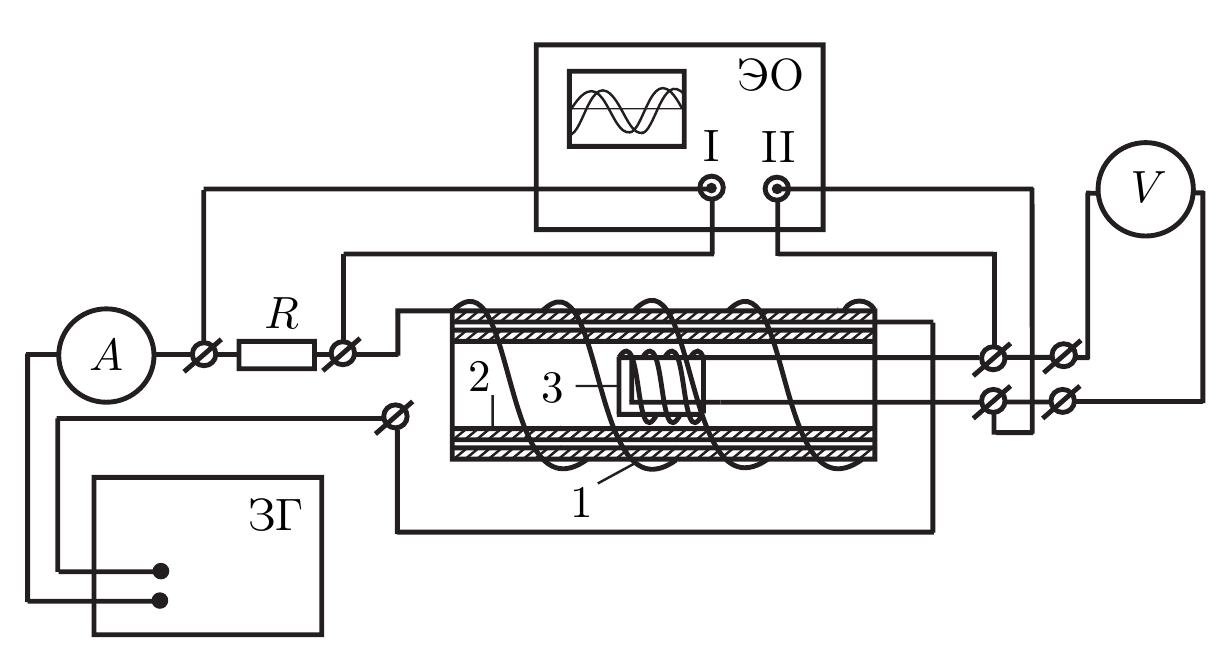
\includegraphics[width=0.48\textwidth]{ustanovka}
\end{center}
\noindent \textbf{Принцип измерений:} \\
Переменное магнитное поле создаётся с помощью соленоида 1, намотанного на цилиндрический каркас 2. \\
(ЗГ) генерирует синусоидальный сигнам с частотой $\nu$. \\
Внутри каркаса расположен медный экран 3 в виде полового цилиндра. \\
Амперметр A снимает показания действующего силы тока $I$ в цепи соленоида. \\
Вольтметр V снимает показания действующего напряжения $U$ на измерительной катушке. \\
Осциллограф (ОЭ) используется для измерения сдвига фаз между током в цепи соленоида и напряжением на измерительной катушке. \\

\noindent \textbf{Измерительные приборы:} \\
Генератор сигналов АКИП-3420ю \\
Двухканальный осциллограф GOS-620 \\

\noindent \textbf{Параметры установки:} \\
Диаметр цилиндра $2a$ = 45 мм \\
Толщина стенки цилиндра $h$ = 1.5 мм \\
$\sigma_{\nu} = 0.01 \ \textup{Гц} \ \textup{(Приборная погрешности)}$ \\
$\sigma_V = 0.0001 \ \textup{В} \ \textup{(Приборная погрешности)}$ \\
$\sigma_I = 0.00001 \ \textup{А} \ \textup{(Приборная погрешности)}$ \\

\newpage

% Магнитное поле внутри цилиндра измеряется катушкой 3. Напряжение на катушке
% пропорционально производной $\dot{B_1}(t)$
% \begin{equation*}
%     U(t) \propto \dot{B_1}(t) = -i\omega H_1 e^{i\omega t}
% \end{equation*}
% Поле внутри цилиндра пропорциональна току через соленоид
% \begin{equation*}
%     B_0(t) \propto I(t)
% \end{equation*}
% Отсюда несложно увидеть, что
% \begin{equation}
%     \frac{\abs{H_1}}{\abs{H_0}} = c \cdot \frac{U}{\nu I} = c \xi
%     \label{eq:otnoshenie_amplitud}
% \end{equation}
% \vspace{0.3cm}

% где константу можно определить из условия $\abs{H_1}/\abs{H_2} \rightarrow 1$ при
% $\nu \rightarrow 0$.

% \vspace{0.3cm}

% При измерениях разности фаз нужно учесть, что первый сигнал на осциллографе
% пропорционален магнитному полю снаружи, а второй пропорционален производному
% поля внутри цилиндра по времени. Вследствие этого набегает дополнительная фаза $\pi/2$,
% которую надо вычесть при измерениях.

% \newpage
% \section{Ход работы}

% Проводимость порядка $\sigma \sim 5\cdot 10^7 \textup{См}/\textup{м}$. Получаем оценку для частоты, при которой
% глубина проникновения равна толщине стенок цилиндра $\nu_h = 2250 \textup{Гц}$.

% \vspace{0.5cm}

% \noindent \textbf{В области низкий частот} (от 0,01 $\nu_h$ до 0,05 $\nu_h$) \textbf{измерим зависимость отношения} $\xi = U/\nu I$ \textbf{от частоты:}

% \[ \frac{1}{\xi^2} = \frac{\nu^2 I^2}{U^2}, \quad \varepsilon_{\xi^2}^2 = 4\varepsilon_{\nu}^2 + 4\varepsilon_{I}^2 + 4 \varepsilon_{U}^2 \]
% \[\sigma_{\nu^2} = 2\nu \sigma_{\nu}\]

% \begin{center}
%     \begin{tabular}{|c|c|c|c|c|c|}
%         \hline
%         N  & $\nu$, Гц & $U$, В & $I$, А   & $\nu^2, \ \textup{Гц}^2$ & $\frac{1}{\xi^2}$ \\ \hline
%         1  & 22.50     & 0.0946 & 0.22186  & $506.25   \pm 0.45$ & $2784 \pm 6$ \\ \hline
%         2  & 30.00     & 0.1244 & 0.22078  & $900.0    \pm 0.6 $ & $2835 \pm 5$ \\ \hline
%         3  & 40.00     & 0.1621 & 0.21853  & $1600.0   \pm 0.8 $ & $2907 \pm 4$ \\ \hline
%         4  & 50.00     & 0.1970 & 0.21573  & $2500.0   \pm 1.0 $ & $2997 \pm 3$ \\ \hline
%         5  & 60.00     & 0.2289 & 0.21257  & $3600.0   \pm 1.2 $ & $3104 \pm 3$ \\ \hline
%         6  & 70.00     & 0.2576 & 0.20920  & $4900.0   \pm 1.4 $ & $3231 \pm 3$ \\ \hline
%         7  & 80.00     & 0.2833 & 0.20578  & $6400.0   \pm 1.6 $ & $3376.7 \pm 2.5$ \\ \hline
%         8  & 90.00     & 0.3060 & 0.20237  & $8100.0   \pm 1.8 $ & $3542.7 \pm 2.5$ \\ \hline
%         9  & 100.00    & 0.3261 & 0.19901  & $10000.0  \pm 2.0 $ & $3724.3 \pm 2.4$ \\ \hline
%         10 & 112.50    & 0.3478 & 0.19507  & $12656.25 \pm 2.25$ & $3981.3 \pm 2.4$ \\ \hline
%     \end{tabular}
% \end{center}

% 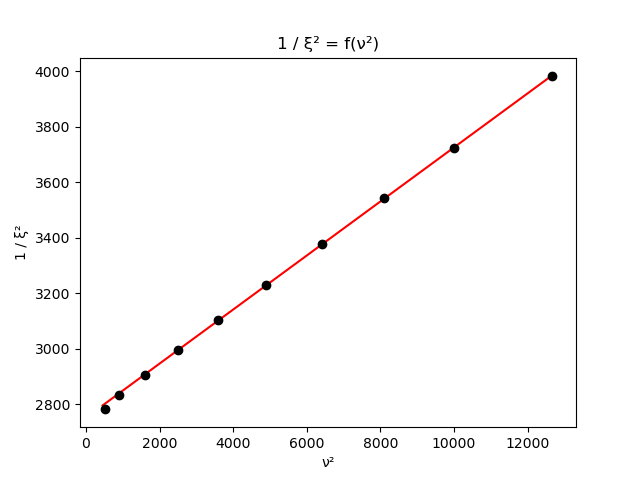
\includegraphics[width=\linewidth]{data2_graphic.png}


% \[\frac{1}{\xi^2} = f(\nu^2)\]
% \[\frac{1}{\xi^2} = k_{\frac{1}{\xi^2}} \cdot \nu^2 + b_{\frac{1}{\xi^2}}\]
% \[k_{\frac{1}{\xi^2}} = (0.0973 \pm 0.0003) \ \frac{1}{\textup{Ом}^2} \]
% \[b_{\frac{1}{\xi^2}} = (2753 \pm 3) \ \frac{\textup{Гц}^2}{\textup{Ом}^2}\]
% \[\textup{Их (7)} \rightarrow k_{\frac{1}{\xi^2}} = \frac{(\pi ah\sigma \mu_0)^2}{\xi_0^2} \quad \rightarrow \quad \sigma = \frac{ \xi_0 \sqrt{k_{\frac{1}{\xi^2}}} }{\pi a h \mu_0} \quad \quad \sigma_{\sigma}^{err} = \sigma \sqrt{\left ( \frac{\sigma_{\xi_0}^{err}}{\xi_0}\right )^2 + \left ( \frac{\sigma_k^{err}}{k}\right )^2}\]
% \[b_{\frac{1}{\xi^2}} = \frac{1}{\xi_0^2} \quad \rightarrow \quad \xi_0 = \frac{1}{\sqrt{b_{\frac{1}{\xi_0^2}}}} \quad \quad \sigma_{\xi_0}^{err} = \frac{1}{2} \frac{\xi_0}{b_{\frac{1}{\xi_0^2}}} \cdot \sigma_{b_{\frac{1}{\xi_0^2}}}^{err}\]
% \[\xi_0 = (0.0191 \pm 0.0003) \ \frac{\textup{Ом}}{\textup{Гц}} \]
% \[\sigma = (5.03 \pm 0.17) \cdot 10^7 \ \frac{\textup{Сименс}}{\textup{м}}\]

% % \newpage % // NOTE
% \vspace{1cm}
% \textbf{Исследуем зависимость зависимость фазы} $\psi$ \textbf{от частоты} $\nu$ (в диапазоне $0.05 \nu_{h}$ до $0.5 \nu_{h})$:

% \[tg(\psi) = f(\nu) \quad \sigma_{tg(\psi)} = \left( \frac{\partial tg\psi}{\partial \psi}\right) \sigma_{\psi} = \frac{\sigma_{\psi}}{\cos^2\psi}\]
% \[\psi = \Delta \varphi - \frac{\pi}{2} \quad \Delta \varphi = \frac{x}{x_0} \pi \quad \varepsilon_{\Delta \varphi} = \sqrt{\varepsilon^2_x + \varepsilon^2_{x_0}}\]

% \[\sigma_{\nu} = 0.1 \ \textup{Гц} \ \textup{(Приборная погрешности)}\]
% \begin{center}
%     \begin{tabular}{|c|c|c|c|}
%         \hline
%         N  & $\nu$, Гц  & $\Delta \varphi - \frac{\pi}{2}$ & $tg\psi$ \\ \hline
%         1  & $ 112.5  $ & $ (0.16 \pm 0.06)\pi           $ & $ 0.55 \pm 0.19 $ \\ \hline
%         2  & $ 122.5  $ & $ (0.22 \pm 0.07)\pi           $ & $ 0.83 \pm 0.23 $ \\ \hline
%         3  & $ 130.0  $ & $ (0.25 \pm 0.07)\pi           $ & $ 0.99 \pm 0.23 $ \\ \hline
%         4  & $ 140.0  $ & $ (0.29 \pm 0.09)\pi           $ & $ 1.29 \pm 0.3  $ \\ \hline
%         5  & $ 150.0  $ & $ (0.27 \pm 0.08)\pi           $ & $ 1.13 \pm 0.3  $ \\ \hline
%         6  & $ 160.0  $ & $ (0.29 \pm 0.09)\pi           $ & $ 1.3  \pm 0.3  $ \\ \hline
%         7  & $ 225.5  $ & $ (0.31 \pm 0.10)\pi           $ & $ 1.5  \pm 0.4  $ \\ \hline
%         8  & $ 300.0  $ & $ (0.34 \pm 0.09)\pi           $ & $ 1.8  \pm 0.5  $ \\ \hline
%         9  & $ 400.0  $ & $ (0.39 \pm 0.09)\pi           $ & $ 2.8  \pm 0.5  $ \\ \hline
%         10 & $ 500.0  $ & $ (0.40 \pm 0.10)\pi           $ & $ 3.1  \pm 0.6  $ \\ \hline
%         11 & $ 600.0  $ & $ (0.43 \pm 0.10)\pi           $ & $ 4.5  \pm 0.8  $ \\ \hline
%         12 & $ 700.0  $ & $ (0.44 \pm 0.10)\pi           $ & $ 5.2  \pm 0.9  $ \\ \hline
%         % 13 & $ 800.0  $ & $ (0.47 \pm 0.10)\pi           $ & $ 10.6 \pm 0.3  $ \\ \hline
%         % 14 & $ 900.0  $ & $ (0.48 \pm 0.11)\pi           $ & $ 15.9 \pm 0.4  $ \\ \hline
%         % 15 & $ 1124.0 $ & $ (0.49 \pm 0.13)\pi           $ & $ 31.8 \pm 0.5  $ \\ \hline
%     \end{tabular}
% \end{center}

% 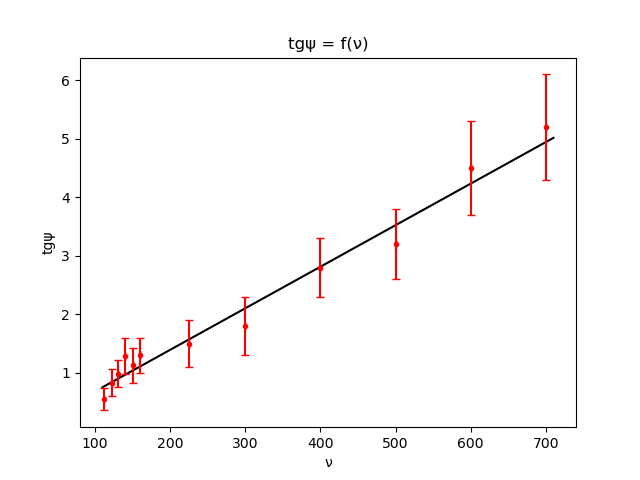
\includegraphics[width=\linewidth]{data_tgpsi.png}

% % \newpage % // NOTE

% \[tg\psi = k_{tg\psi} \nu + b_{tg \psi}\]
% \[k_{tg\psi} = (0.0071 \pm 0.0005) \ \textup{Гц}^{-1}\]
% \[b_{tg\psi} = (-0.03 \pm 0.11)\]
% \[\textup{Из (8)}\rightarrow \sigma = \frac{k_{tg\psi}}{\pi a h \mu_0} \quad \sigma_{\sigma}^{err} = \frac{\sigma}{k_{tg\psi}} \cdot \sigma_{k_{tg\psi}}^{err}\]
% \[\sigma = (5.4 \pm 0.3) \cdot 10^7 \ \frac{\textup{Сименс}}{\textup{м}}\]

% % \newpage % // NOTE

% \vspace{1cm}
% \textbf{Исследуем зависимость сдвига фаз} $\psi - \frac{\pi}{2}$ \textbf{от частоты} $\nu$:

% \[\psi - \frac{\pi}{4} = f(\sqrt{\nu}) \quad \sigma_{\sqrt{\nu}} = \frac{\sigma_{\nu}}{2\sqrt{\nu}} \quad \sigma_{\nu} = 10 \textup{Гц}\]


% \begin{center}
%     \begin{tabular}{|c|c|c|c|}
%         \hline
%         N & $\nu$, Гц  & $ \sqrt{\nu}        $ & $\psi - \frac{\pi}{4}$ \\ \hline
%         1  & $ 1120  $ & $ 33.46  \pm 0.15 $ & $ (0.32 \pm 0.05)\pi $ \\ \hline
%         2  & $ 2000  $ & $ 44.72  \pm 0.11 $ & $ (0.34 \pm 0.06)\pi $ \\ \hline
%         3  & $ 4000  $ & $ 63.25  \pm 0.08 $ & $ (0.46 \pm 0.08)\pi $ \\ \hline
%         4  & $ 6000  $ & $ 77.46  \pm 0.06 $ & $ (0.47 \pm 0.08)\pi $ \\ \hline
%         5  & $ 8000  $ & $ 89.44  \pm 0.05 $ & $ (0.54 \pm 0.10)\pi $ \\ \hline
%         6  & $ 10000 $ & $ 100.00 \pm 0.05 $ & $ (0.58 \pm 0.11)\pi $ \\ \hline
%         7  & $ 12000 $ & $ 109.54 \pm 0.05 $ & $ (0.68 \pm 0.14)\pi $ \\ \hline
%         8  & $ 14000 $ & $ 118.32 \pm 0.04 $ & $ (0.78 \pm 0.16)\pi $ \\ \hline
%         9  & $ 16000 $ & $ 126.49 \pm 0.04 $ & $ (0.81 \pm 0.18)\pi $ \\ \hline
%         % 10 & $ 18000 $ & $ (134.16 \pm 0.04) $ & $ (1.02 \pm 0.22)\pi $ \\ \hline
%     \end{tabular}
% \end{center}

% % 134.16 0.04 1.02 0.22

% 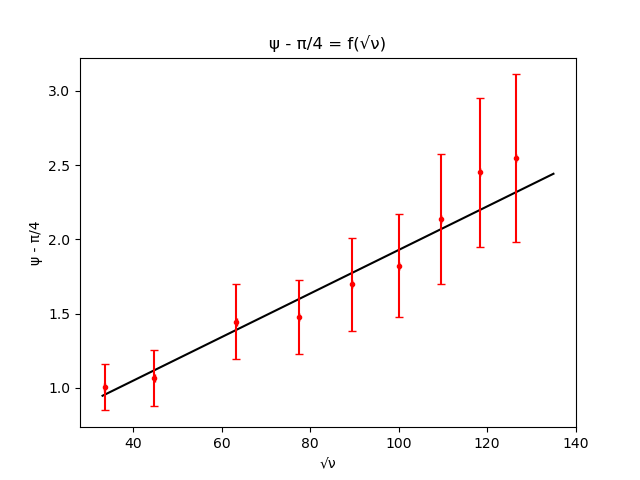
\includegraphics[width=\linewidth]{psi.png}

% \[\psi - \frac{\pi}{4}= k_{\psi} \sqrt{\nu} + b_{\psi}\]
% \[\textup{Из (9)} \rightarrow k_{\psi} = h\sqrt{\pi \sigma \mu_0} \rightarrow \sigma = \frac{1}{\pi \mu_0} \cdot \left (\frac{k_{\psi}}{h} \right ) ^ 2 \quad \sigma_{\sigma}^{err} = 2\sigma_{k_{\psi}}^{err} \cdot \frac{\sigma}{k_{\psi}}\]
% \[k_{\psi} = (0.0157 \pm 0.0015) \ \textup{Гц}^{-\frac{1}{2}}\]
% \[b_{\psi} = (0.41 \pm 0.11)\]
% \[\sigma = (5.5 \pm 0.5) \cdot 10^7 \ \frac{\textup{Сименс}}{\textup{м}}\]

% % //FIXME блять тут было 2.8

% % \newpage % // NOTE
% \vspace{1cm}
% \textbf{Исследуем зависимость индуктивности} $L$ \textbf{от частоты} $\nu$:

% % // FIXME исправить L * 10^3

% \[\varepsilon_{\nu} = 0.01\]
% \begin{center}
%     \begin{tabular}{|c|c|c|}
%         \hline
%         N  & $\nu$ & $L,\  10^{-3}$Гн \\ \hline
%         1  & $ 50.0  \pm 0.5 $ & $ 9.88 \pm 0.05 $ \\ \hline
%         2  & $ 150   \pm 1.5 $ & $ 7.25 \pm 0.05 $ \\ \hline
%         3  & $ 250   \pm 2.5 $ & $ 5.36 \pm 0.05 $ \\ \hline
%         4  & $ 400   \pm 4   $ & $ 4.08 \pm 0.05 $ \\ \hline
%         5  & $ 500   \pm 5   $ & $ 3.69 \pm 0.05 $ \\ \hline
%         6  & $ 600   \pm 6   $ & $ 3.46 \pm 0.05 $ \\ \hline
%         7  & $ 800   \pm 8   $ & $ 3.21 \pm 0.05 $ \\ \hline
%         8  & $ 1500  \pm 15  $ & $ 2.97 \pm 0.05 $ \\ \hline
%         9  & $ 4000  \pm 40  $ & $ 2.89 \pm 0.05 $ \\ \hline
%         10 & $ 7500  \pm 75  $ & $ 2.92 \pm 0.01 $ \\ \hline
%         11 & $ 12000 \pm 120 $ & $ 3.05 \pm 0.01 $ \\ \hline
%         12 & $ 16200 \pm 162 $ & $ 3.31 \pm 0.01 $ \\ \hline
%         13 & $ 20000 \pm 200 $ & $ 3.71 \pm 0.01 $ \\ \hline
%     \end{tabular}
% \end{center}

% 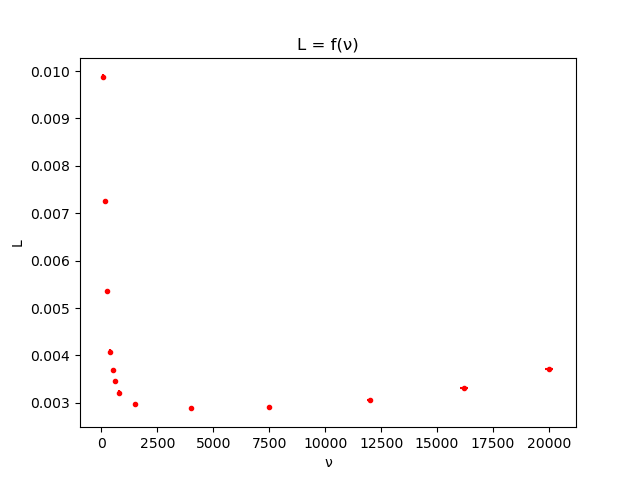
\includegraphics[width=\linewidth]{L_nu.png}

% \[f(L, L_{min}, L_{max}) = \frac{L_{max} - L_{}}{L - L_{min}} \]
% \[\sigma_f^2 = \left ( \frac{L_{max} - L_{min}}{\left ( L - L_{min} \right )^2} \right )^2 \sigma_L^2 + \left ( \frac{L_{max} - L}{\left ( L - L_{min} \right )^2}\right )^2 \sigma_{L_{min}}^2 + \left ( \frac{1}{L - L_{min}}\right )^2 \sigma_{L_{max}}^2 \]
% \[L_{min}= (2.89 \pm 0.05) \ \textup{Гн} \quad \quad L_{max} = (9.88 \pm 0.05) \ \textup{Гн}\]

% \begin{center}
%     \begin{tabular}{|c|c|c|}
%         \hline
%         N & $\nu^2$                      & $f(L, L_{min}, L_{max})$ \\ \hline
%         1  & $ 2500 \pm 50             $ & $0.883 \pm 0.010$ \\ \hline
%         2  & $ (225 \pm 5) \cdot 10^2  $ & $1.415 \pm 0.023$ \\ \hline
%         3  & $ (625 \pm 13) \cdot 10^2 $ & $2.50 \pm 0.07$ \\ \hline
%         4  & $ (160 \pm 3) \cdot 10^3  $ & $5.2 \pm 0.3$ \\ \hline
%         5  & $ (250 \pm 5) \cdot 10^3  $ & $7.7 \pm 0.7$ \\ \hline
%         6  & $ (360 \pm 7) \cdot 10^3  $ & $10.8 \pm 1.5$ \\ \hline
%         7  & $ (640 \pm 13) \cdot 10^3 $ & $19 \pm 4$ \\ \hline
%         % 8  & $ (225 \pm 5) \cdot 10^4  $ & $77 \pm 80$ \\ \hline
%         % 9  & $ (560 \pm 11) \cdot 10^5 $ & $206 \pm 400$ \\ \hline
%         % 10 & $ (144 \pm 3) \cdot 10^6  $ & $39 \pm 14$ \\ \hline
%         % 11 & $ (262 \pm 5) \cdot 10^6  $ & $14.7 \pm 1.9$ \\ \hline
%         % 12 & $ (400 \pm 8) \cdot 10^6  $ & $7.5 \pm 0.5$ \\ \hline
%     \end{tabular}
% \end{center}

% 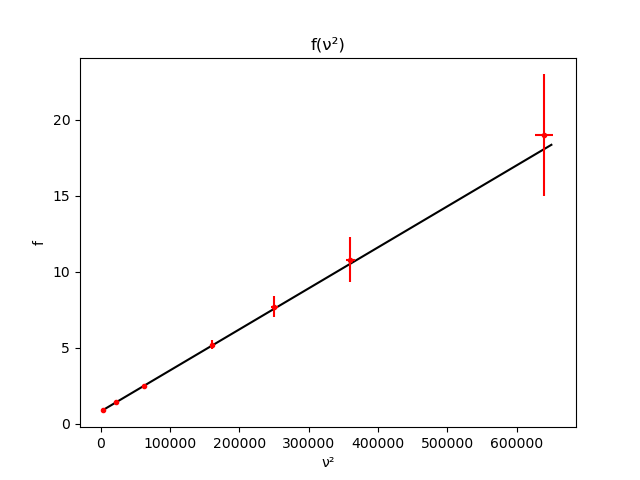
\includegraphics[width=\linewidth]{f_nu2.png}

% \[\textup{Из (10)} \rightarrow f = k_{f} \nu^2 = (\pi a h \mu_0 \sigma)^2 \cdot \nu^2 \rightarrow \sigma = \frac{\sqrt{k_f}}{\pi a h \mu_0} \quad \sigma_{\sigma}^{err} = \frac{1}{2} \frac{\sigma}{k_f} \cdot \sigma_k^{err}\]
% \[k_f = (2.699 \pm 0.017) \cdot 10^{-5} \ \textup{Гц}^{-1} \rightarrow \sigma = ( 4.387 \pm 0.014 ) \cdot 10^7\]

% % 2250000 50000 77 80
% % 56000000 1100000 206 400
% % 144000000 3000000 39 14
% % 262000000 5000000 14.7 1.9
% % 400000000 8000000 7.5 0.5

% % \newpage

% \vspace{1cm}
% \section{Вывод}
% Мы измерили проводимость материала цилиндра 4 разными способами. Сравним эти данные
% между собой

% \begin{table}[!h]
%     \begin{center}
%         \begin{tabular}{lrrr}
%             Метод измерения & $\sigma, 10^{7} \textup{См/м}$ & $\sigma_{\sigma}^{err}, 10^{7} \textup{См/м}$ & $\varepsilon_{\sigma}$\\
%             \toprule
%             Отношение амплитуд             & 5.03  & 0.17  & 0.03  \\
%             Разности фаз (низкие частоты)  & 5.4   & 0.3   & 0.06  \\
%             Разности фаз (высокие частоты) & 5.5   & 0.5   & 0.09  \\
%             Индуктивность                  & 4.387 & 0.014 & 0.003 \\
%         \end{tabular}
%     \end{center}
% \end{table}

% Для данной марки меди проводимость состовляет $\sigma_{точн.} = 5.62\cdot10^{7} \textup{См/м}$.

% Самым неточным оказался метод измерения через разность фаз при высоких частотах.
% Как видим, при частотах $\sim 5 \textup{кГц}$
% зависимость индуктивности не описывается теорией, следовательно, при этих частотах не должна работать и остальная теория.
% Как результат, зависимость разности фаз от корня частоты уже не описывается линейной
% зависимостью.

% Погрешность измерения проводимости через разность фаз при низких частотах в основном
% связана с погрешностью измерения самой разности фаз, т.к. погрешность последней
% возрастает в несколько раз при подсчете тангенса угла.

% % 640000 13000 19 4

% \end{document}

\end{document}
